\section{Используемые технологии}
\label{sec:techs:intro}

Выбор технологий является важным предварительным этапом разработки сложных информационных систем. Платформа и язык программирования, на котором будет реализована система, заслуживает большого внимания, так как множество исследований показали, что выбор языка программирования значительно влияет на производительность труда программистов и качество создаваемого ими кода~\cite[c.~59]{mcconnell_2005}.

На выбор технологий повлияли следующие факторы:
\begin{itemize}
\item программное средство должно быть выполнено в виде клиент"=серверного приложения;
\item разрабатываемое ПО должно работать на операционных системах Linux, MacOS и Windows;
\item разработчик имеет опыт работы с объектно"=ориентированными и функциональными языками программирования.
\end{itemize}

\subsection{Язык программирования Scala}
\label{sub:techs:scala}
Scala — мультипарадигмальный, компилируемый, строго типизированный язык программирования, спроектированный кратким и безопасным для простого и быстрого создания компонентного программного обеспечения, сочетающий возможности функционального и объектно-ориентированного программирования~\cite{wiki_scala}.

Scala поддерживает объектно-ориентированную и функциональную парадигмы программирования, но доминирующей является объектно-ориентированная. Язык был выпущен для общего пользования на платформе JVM и .NET, так же создан LLVM-компилятор (Scala Native) и транслятор в JavaScript (ScalaJS).

Отличительные особенности языка Scala:
\begin{itemize}
  \item лаконичность. Код на Scala в средней вдвое короче кода на Java.
  \item открытый исходный код. Код стандартной библиотеки опубликован к открытом доступе на портале GitHub и любой желающий, при наличии желания и способностей, может стать участником проекта.
  \item высокий уровень абстракции. В стандартной библиотеке реализованы большинство типичных операции над строками и коллекциями, в частности итерация по элементам коллекции инкапсулирована в методах map, filter, flatMap. Так же выражение for трансформируется в вызов выше описанных методов, что позволяет использовать в нем пользовательские контейнеры и типы данных. 
  \item платформонезависимость. Код языка компилируется в JVM байт-код и может исполняться на любой платформе поддерживающей JVM.
  \item строгая система типов. Позволяет выявить многое ошибки еще на стадии компиляции.
  \item объектно-ориентированность. Язык поддерживает основные концепции объектно-ориентированного программирование (наследование, инкапсуляция, полиморфизм).
  \item функциональность. Язык поддерживает основные концепции функционального программирование (функции высших порядков, сопоставление с образцов, <<ленивые>> вычисления).
  \item расширяемость. В языке присутствуют механизм (неявные преобразования) позволяющий расширять функционал стандартных классов и сторонних библиотек.
  \item использование Java-кода. Возможно использовать не только библиотеки написанные на Java, но и классы написанные на Java в Scala-проекте, но отсутствует полная обратная совместимость.
  \item широкий набор библиотеки. Стандартная библиотека Scala содержит классы для работы с вводом-выводом, регулярными выражениями, параллельной обработки, работы со строками, коллекции. Так же существует большое количество сторонних библиотек.
\end{itemize}

Основываясь на выше перечисленных факторах было принято решение использовать в качестве основного языка программирования Scala как современный, активно набирающий популярность язык поддерживающий функциональную и объектно"=ориентированную парадигмы программирования.

Далее приводится подробная характеристика языка программирования.

\subsubsection{Объектно-ориентированное программирование}
Объектно-ориентированная парадигма программирования играет в языке важную роль. Стандартная библиотека языка реализована в виде набора классов и примесей, а так же модульность обеспечивается классами и пакетами~\cite{horsman_scala}.

Особенности Scala с точки зрения объектно"=ориентированной парадигмы:
\begin{itemize}
  \item статическая сильная полная типизация с автоматическим выведением типов;
  \item наследование, в том числе использование примесей (Traits);
  \item полиморфизм;
  \item инкапсуляция;
  \item конструкторы, деструкторы;
  \item все операторы (+, -, *) являются методами;
  \item гибкое управление доступом к полям и методам;
  \item метапрограммирование;
  \item объекты компаньоны (используются для инкапсуляции статических полей и методов).
\end{itemize}

\subsubsection{Функциональное программирование}
Особенности Scala с точки зрения функциональной парадигмы:
\begin{itemize}
  \item функции высших порядков;
  \item функции объект первого класса;
  \item оптимизация хвостовой рекурсии;
  \item сопоставление с образцов;
  \item поддержка неизменяемых структур данных;
  \item функциональные комбинаторы и композиции;
  \item частичное применение функции;
  \item <<ленивые>> вычисления;
  \item структурное переиспользование неизменяемых коллекций.
\end{itemize}

\subsection{Фреймворк Akka}
\label{sec:techs:akka}

Akka - набор прикладных библиотек (фреймворк) предоставляющий высокоуровневый интерфейс для разработки, развертывания и отладки систем акторов.

Основными достоинствами фреймворка Akka являются:
\begin{itemize}
  \item простота интерфейса, высокая степень абстракции;
  \item устойчивость к отказам. Благодаря механизму супервизор;
  \item масштабируемость. Проста добавления акторов в систему и развертывания компонентов на другой машине;
  \item высокая скорость работы и степень параллелизма. Благодаря использованию модели акторов;
  \item минимально количество блокирующих операций. Отсутствие общего изменяемого состояния.
\end{itemize}

Перечисленные достоинства, в особенности устойчивой к отказам и простота масштабирования, являются крайне важными при реализации архитектуры на основе микросервисов. Исходя из выше перечисленного для обеспечения параллельной обработки данных будет использоваться набор прикладных библиотек (фреймворк) Akka. 

\begin{figure}[ht]
    \centering
    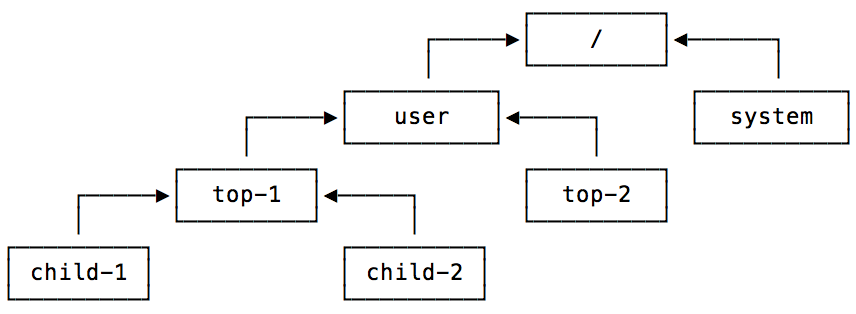
\includegraphics[width=0.7\textwidth]{figures/actors_hier.png}
    \label{fig:techs:akka:actor_hierar}
    \caption{Иерархия акторов}
\end{figure}

\subsubsection{Модель акторов}
\label{sec:techs:akka:actor_model}
Модель акторов - модель параллельных вычислений, основанная на взаимодействии изолированных примитивов взаимодействующих по средствам получения и отправки сообщений. Впервые была предложена в 1973 году~\cite{hewitt_bishop_steiger_actor_model}.

Основным понятием данной модели является «актор». Согласно модели актор лишен состояния и информации о структуре системы (количество братьев и родителей). 

\begin{figure}[ht]
    \centering
    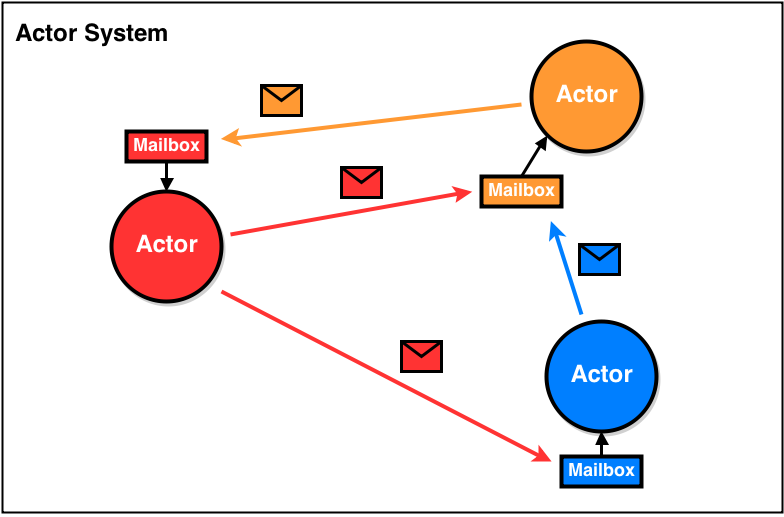
\includegraphics[width=0.7\textwidth]{figures/actor_model.png}
    \label{fig:techs:akka:actor_model:comulication}
    \caption{Пример взаимодействия акторов}
\end{figure}

\subsection{Фреймворк Spray}
\label{sec:techs:spray}

Spray - набор прикладных библиотек (фреймворк) предназначенного реализации веб-приложений.

Данный фреймворк базируется на описанном выше фреймворке Akka и реализует асинхронное распределение запросов пользователя на иерархию акторов. 

Основными достоинствами фреймворка Spray являются:
\begin{itemize}
  \item полная асинхронность, отсутствие блокировок (весь интерфейс полностью асинхронный);
  \item высокая производительность (используются специальные низкоуровневые компоненты);
  \item модульность (весь интерфейс полностью асинхронный);
  \item легковесность (включаются только необходимые модули);
\end{itemize}

Использование данного фреймворка позволит упростить разработку, отладку и последующее сопровождения благодаря использования одной концепции с предыдущим фреймворком.
Исходя из выше перечисленного для реализации серверной часть приложения будет использоваться набор прикладных библиотек (фреймворк) Spray.